\documentclass[12pt]{article}
\usepackage{fontspec}
\usepackage{fullpage}
\usepackage{hyperref}
\hypersetup{bookmarks=true,colorlinks=true,linkcolor=red,citecolor=blue,filecolor=magenta,urlcolor=cyan}
\usepackage{amsmath}
\usepackage{amssymb}
\usepackage{mathtools}
\usepackage{unicode-math}
\usepackage{tabularray}
\usepackage{tabularx}
\usepackage{booktabs}
\usepackage{caption}
\usepackage{graphics}
\usepackage{svg}
\usepackage{float}
\usepackage{enumitem}
\usepackage{adjustbox}
\usepackage{filecontents}
\usepackage[backend=bibtex]{biblatex}
\usepackage{url}
\setmathfont{Latin Modern Math}
\newcommand{\gt}{\ensuremath >}
\newcommand{\lt}{\ensuremath <}
\newlist{symbDescription}{description}{1}
\setlist[symbDescription]{noitemsep, topsep=0pt, parsep=0pt, partopsep=0pt}
\newcommand{\resizeExpression}[1]{
  \adjustbox{max width=\linewidth}{$#1$}
}
\bibliography{bibfile}
\title{Software Requirements Specification for Binary Star System Simulator}
\author{Xinlu Yan}
\begin{document}
\maketitle
\tableofcontents
\newpage
\section{Reference Material}
\label{Sec:RefMat}
This section records information for easy reference.

\subsection{Table of Units}
\label{Sec:ToU}
The unit system used throughout is SI (Système International d'Unités). In addition to the basic units, several derived units are also used. For each unit, the \hyperref[Table:ToU]{Table of Units} lists the symbol, a description, and the SI name.

\begin{longtblr}
[caption={Table of Units}]
{colspec={l l l}, rowhead=1, hline{1,Z}=\heavyrulewidth, hline{2}=\lightrulewidth}
\textbf{Symbol} & \textbf{Description} & \textbf{SI Name}
\\
${\text{J}}$ & energy & joule
\\
${\text{kg}}$ & mass & kilogram
\\
${\text{m}}$ & length & metre
\\
${\text{N}}$ & force & newton
\\
${\text{s}}$ & time & second
\label{Table:ToU}
\end{longtblr}
\subsection{Table of Symbols}
\label{Sec:ToS}
The symbols used in this document are summarized in the \hyperref[Table:ToS]{Table of Symbols} along with their units. Throughout the document, symbols in bold will represent vectors, and scalars otherwise. The symbols are listed in alphabetical order. For vector quantities, the units shown are for each component of the vector.

\begin{longtblr}
[caption={Table of Symbols}]
{colspec={l l l}, rowhead=1, hline{1,Z}=\heavyrulewidth, hline{2}=\lightrulewidth}
\textbf{Symbol} & \textbf{Description} & \textbf{Units}
\\
${a_{\text{x}1}}$ & X-acceleration of the first star & $\frac{\text{m}}{\text{s}^{2}}$
\\
${a_{\text{x}2}}$ & X-acceleration of the second star & $\frac{\text{m}}{\text{s}^{2}}$
\\
${a_{\text{y}1}}$ & Y-acceleration of the first star & $\frac{\text{m}}{\text{s}^{2}}$
\\
${a_{\text{y}2}}$ & Y-acceleration of the second star & $\frac{\text{m}}{\text{s}^{2}}$
\\
$\symbf{a}\text{(}t\text{)}$ & Acceleration & $\frac{\text{m}}{\text{s}^{2}}$
\\
$E$ & Energy & ${\text{J}}$
\\
$\symbf{F}$ & Force & ${\text{N}}$
\\
${\symbf{F}_{\symbf{g}}}$ & Force of gravity & ${\text{N}}$
\\
$G$ & Gravitational constant & $\frac{\text{m}^{3}}{\text{kg}\text{s}^{2}}$
\\
$i$ & Index & --
\\
$m$ & Mass & ${\text{kg}}$
\\
${m_{1}}$ & Mass of the first star & ${\text{kg}}$
\\
${m_{2}}$ & Mass of the second star & ${\text{kg}}$
\\
${m_{\text{max}}}$ & Maximum stellar mass & ${\text{kg}}$
\\
${m_{\text{min}}}$ & Minimum stellar mass & ${\text{kg}}$
\\
$n$ & Number of bodies & --
\\
$\symbf{p}\text{(}t\text{)}$ & Position & ${\text{m}}$
\\
${r_{12}}$ & Separation distance & ${\text{m}}$
\\
${r_{\text{max}}}$ & Maximum initial distance from origin & ${\text{m}}$
\\
$t$ & Time & ${\text{s}}$
\\
${t_{\text{final}}}$ & Final time & ${\text{s}}$
\\
${t_{\text{max}}}$ & Maximum simulation time & ${\text{s}}$
\\
${v_{\text{max}}}$ & Maximum initial speed & $\frac{\text{m}}{\text{s}}$
\\
${v_{\text{x}1}}$ & X-velocity of the first star & $\frac{\text{m}}{\text{s}}$
\\
${{v_{\text{x}1}}^{0}}$ & Initial x-velocity of the first star & $\frac{\text{m}}{\text{s}}$
\\
${v_{\text{x}2}}$ & X-velocity of the second star & $\frac{\text{m}}{\text{s}}$
\\
${{v_{\text{x}2}}^{0}}$ & Initial x-velocity of the second star & $\frac{\text{m}}{\text{s}}$
\\
${v_{\text{y}1}}$ & Y-velocity of the first star & $\frac{\text{m}}{\text{s}}$
\\
${{v_{\text{y}1}}^{0}}$ & Initial y-velocity of the first star & $\frac{\text{m}}{\text{s}}$
\\
${v_{\text{y}2}}$ & Y-velocity of the second star & $\frac{\text{m}}{\text{s}}$
\\
${{v_{\text{y}2}}^{0}}$ & Initial y-velocity of the second star & $\frac{\text{m}}{\text{s}}$
\\
$\symbf{v}\text{(}t\text{)}$ & Velocity & $\frac{\text{m}}{\text{s}}$
\\
${x_{1}}$ & X-position of the first star & ${\text{m}}$
\\
${{x_{1}}^{0}}$ & Initial x-position of the first star & ${\text{m}}$
\\
${x_{2}}$ & X-position of the second star & ${\text{m}}$
\\
${{x_{2}}^{0}}$ & Initial x-position of the second star & ${\text{m}}$
\\
${y_{1}}$ & Y-position of the first star & ${\text{m}}$
\\
${{y_{1}}^{0}}$ & Initial y-position of the first star & ${\text{m}}$
\\
${y_{2}}$ & Y-position of the second star & ${\text{m}}$
\\
${{y_{2}}^{0}}$ & Initial y-position of the second star & ${\text{m}}$
\label{Table:ToS}
\end{longtblr}
\subsection{Abbreviations and Acronyms}
\label{Sec:TAbbAcc}
\begin{longtblr}
[caption={Abbreviations and Acronyms}]
{colspec={l l}, rowhead=1, hline{1,Z}=\heavyrulewidth, hline{2}=\lightrulewidth}
\textbf{Abbreviation} & \textbf{Full Form}
\\
A & Assumption
\\
DD & Data Definition
\\
GD & General Definition
\\
GS & Goal Statement
\\
IM & Instance Model
\\
LC & Likely Change
\\
ODE & Ordinary Differential Equation
\\
PS & Physical System Description
\\
R & Requirement
\\
RefBy & Referenced by
\\
Refname & Reference Name
\\
SRS & Software Requirements Specification
\\
TM & Theoretical Model
\\
UC & Unlikely Change
\\
Uncert. & Typical Uncertainty
\label{Table:TAbbAcc}
\end{longtblr}
\section{Introduction}
\label{Sec:Intro}
Binary star systems are common in astronomy. Two stars orbit because of gravity. This software simulates how a binary star system evolves over time.

The following section provides an overview of the software requirements specification (SRS) for Binary Star System Simulator. This section explains the purpose of this document, the scope of the requirements, the characteristics of the intended reader, and the organization of the document.

\subsection{Purpose of Document}
\label{Sec:DocPurpose}
The primary purpose of this document is to record the requirements of BSS. Goals, assumptions, theoretical models, definitions, and other model derivation information are specified, allowing the reader to fully understand and verify the purpose and scientific basis of BSS. With the exception of \hyperref[Sec:SysConstraints]{system constraints}, this SRS will remain abstract, describing what problem is being solved, but not how to solve it.

This document will be used as a starting point for subsequent development phases, including writing the design specification and the software verification and validation plan. The design document will show how the requirements are to be realized, including decisions on the numerical algorithms and programming environment. The verification and validation plan will show the steps that will be used to increase confidence in the software documentation and the implementation. Although the SRS fits in a series of documents that follow the so-called waterfall model, the actual development process is not constrained in any way. Even when the waterfall model is not followed, as Parnas and Clements point out \cite{parnasClements1986}, the most logical way to present the documentation is still to ``fake'' a rational design process.

\subsection{Scope of Requirements}
\label{Sec:ReqsScope}
The scope of the requirements includes two-dimensional , rigid-body mechanics where the only force is gravitational attraction.

\subsection{Characteristics of Intended Reader}
\label{Sec:ReaderChars}
Reviewers of this documentation should have an understanding of undergraduate level 1 physics (Newtonian mechanics), undergraduate level 1 calculus, and ordinary differential equations. The users of BSS can have a lower level of expertise, as explained in \hyperref[Sec:UserChars]{Sec:User Characteristics}.

\subsection{Organization of Document}
\label{Sec:DocOrg}
The organization of this document follows the template for an SRS for scientific computing software proposed by \cite{koothoor2013}, \cite{smithLai2005}, \cite{smithEtAl2007}, and \cite{smithKoothoor2016}. The presentation follows the standard pattern of presenting goals, theories, definitions, and assumptions. For readers that would like a more bottom up approach, they can start reading the \hyperref[Sec:IMs]{instance models} and trace back to find any additional information they require.

The \hyperref[Sec:GoalStmt]{goal statements} are refined to the theoretical models and the \hyperref[Sec:TMs]{theoretical models} to the \hyperref[Sec:IMs]{instance models}.

\section{General System Description}
\label{Sec:GenSysDesc}
This section provides general information about the system. It identifies the interfaces between the system and its environment, describes the user characteristics, and lists the system constraints.

\subsection{System Context}
\label{Sec:SysContext}
\hyperref[Figure:sysCtxDiag]{Fig:sysCtxDiag} shows the system context. A circle represents an entity external to the software, the user in this case. A rectangle represents the software system itself (BSS). Arrows are used to show the data flow between the system and its environment.

\begin{figure}[H]
\begin{center}

\includegraphics[width=\textwidth]{../../../../datafiles/bss/SystemContextFigure.png}
\caption{System Context}
\label{Figure:sysCtxDiag}
\end{center}
\end{figure}
The interaction between the product and the user is through an application programming interface. The responsibilities of the user and the system are as follows:

\begin{itemize}
\item{User Responsibilities}
\begin{itemize}
\item{Provide the physical parameters of the binary star system, including stellar masses, initial positions, and initial velocities, ensuring no errors in the data entry.}
\item{Ensure that consistent units are used for inputs.}
\item{Ensure required \hyperref[Sec:Assumps]{software assumptions} are appropriate for any particular problem input to the software.}
\end{itemize}
\item{BSS Responsibilities}
\begin{itemize}
\item{Detect data type mismatch, such as a string of characters input instead of a floating point number.}
\item{Determine if the inputs satisfy the required physical and software constraints.}
\item{Calculate the required outputs.}
\end{itemize}
\end{itemize}
\subsection{User Characteristics}
\label{Sec:UserChars}
The end user of BSS should have an understanding of undergraduate level 1 physics (Newtonian mechanics), undergraduate level 1 calculus and ordinary differential equations.

\subsection{System Constraints}
\label{Sec:SysConstraints}
There are no system constraints.

\section{Specific System Description}
\label{Sec:SpecSystDesc}
This section first presents the problem description, which gives a high-level view of the problem to be solved. This is followed by the solution characteristics specification, which presents the assumptions, theories, and definitions that are used.

\subsection{Problem Description}
\label{Sec:ProbDesc}
A system is needed to simulate the motion of a binary star system under mutual gravitational interaction.

\subsubsection{Terminology and Definitions}
\label{Sec:TermDefs}
This subsection provides a list of terms that are used in the subsequent sections and their meaning, with the purpose of reducing ambiguity and making it easier to correctly understand the requirements.

\begin{itemize}
\item{Binary star system: A system consisting of two stars that orbit around their common center of mass due to gravitational interaction.}
\item{Star: A massive astronomical object that is treated as a point mass in this context.}
\item{Gravitational interaction: The mutual attractive force between two masses as described by Newtonian gravity.}
\item{Newton's law of universal gravitation: The law stating that every mass attracts every other mass with a force proportional to the product of their masses and inversely proportional to the square of the distance between them.}
\item{Initial conditions: The positions and velocities of the stars at the start of the simulation.}
\item{Trajectory: The path traced by a star in space as a function of time.}
\item{Center of mass: The point representing the average position of the mass distribution of the system.}
\item{Inertial reference frame: A reference frame in which Newton's laws of motion are valid without the introduction of fictitious forces.}
\item{Simulation time span: The duration over which the evolution of the system is computed.}
\end{itemize}
\subsubsection{Physical System Description}
\label{Sec:PhysSyst}
The physical system of BSS, as shown in \hyperref[Figure:bssPhysSys]{Fig:bssPhysSys}, includes the following elements:

\begin{description}[font=\normalfont]
\item[PS1:]{The first star with mass ${m_{1}}$.}
\item[PS2:]{The second star with mass ${m_{2}}$.}
\item[PS3:]{The gravitational interaction between the two stars.}
\end{description}
\begin{figure}[H]
\begin{center}
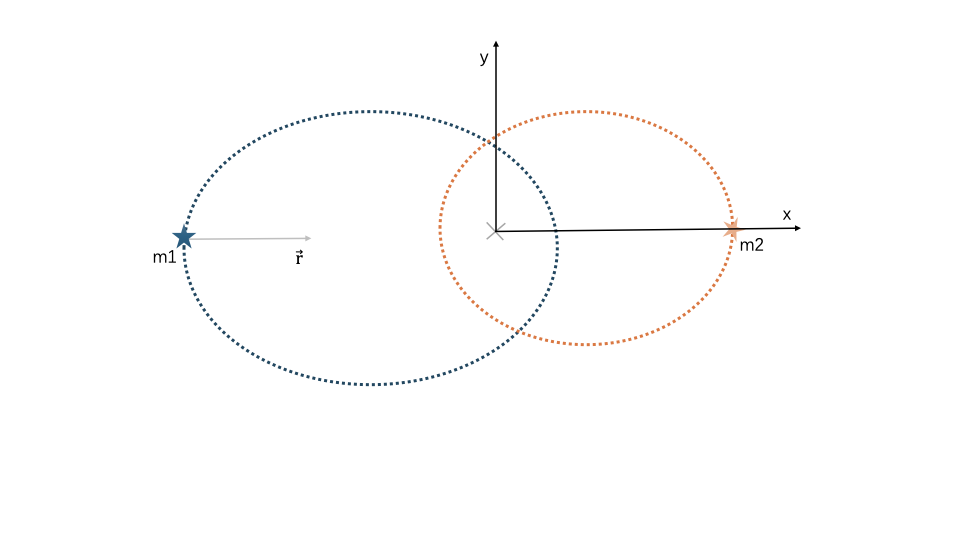
\includegraphics[width=0.6\textwidth]{../../../../datafiles/bss/bss.png}
\caption{The physical system}
\label{Figure:bssPhysSys}
\end{center}
\end{figure}
\subsubsection{Goal Statements}
\label{Sec:GoalStmt}
Given the masses (${m_{1}}$ and ${m_{2}}$), the initial positions (${{x_{1}}^{0}}$, ${{y_{1}}^{0}}$, ${{x_{2}}^{0}}$, ${{y_{2}}^{0}}$), the initial velocities (${{v_{\text{x}1}}^{0}}$, ${{v_{\text{y}1}}^{0}}$, ${{v_{\text{x}2}}^{0}}$, ${{v_{\text{y}2}}^{0}}$), and the simulation time (${t_{\text{final}}}$), the goal statement is:

\begin{description}[font=\normalfont]
\item[positionsOverTime:\phantomsection\label{positionsOverTime}]{Determine the positions of both stars as functions of time over the specified simulation interval.}
\end{description}
\subsection{Solution Characteristics Specification}
\label{Sec:SolCharSpec}
The instance models that govern BSS are presented in the \hyperref[Sec:IMs]{Instance Model Section}. The information to understand the meaning of the instance models and their derivation is also presented, so that the instance models can be verified.

\subsubsection{Assumptions}
\label{Sec:Assumps}
This section simplifies the original problem and helps in developing the theoretical models by filling in the missing information for the physical system. The assumptions refine the scope by providing more detail.

\begin{description}[font=\normalfont]
\item[twoBody:\phantomsection\label{twoBody}]{The system consists of exactly two stars with masses ${m_{1}}$ and ${m_{2}}$ . Perturbations from third-body gravity are ignored. (RefBy: \hyperref[IM:accelY2]{IM:accelY2}, \hyperref[IM:accelY1]{IM:accelY1}, \hyperref[IM:accelX2]{IM:accelX2}, \hyperref[IM:accelX1]{IM:accelX1}, and \hyperref[lcDerivedOutputs]{LC:Derived-Output-Quantities}.)}
\item[isolated:\phantomsection\label{isolated}]{Non-gravitational forces (e.g., drag, thrust, radiation pressure) are neglected; the only interaction modeled is mutual gravity between the two stars (from \hyperref[newtonianGravity]{A:newtonianGravity}). (RefBy: \hyperref[IM:accelY2]{IM:accelY2}, \hyperref[IM:accelY1]{IM:accelY1}, \hyperref[IM:accelX2]{IM:accelX2}, \hyperref[IM:accelX1]{IM:accelX1}, and \hyperref[lcDerivedOutputs]{LC:Derived-Output-Quantities}.)}
\item[newtonianGravity:\phantomsection\label{newtonianGravity}]{The gravitational interaction between the stars is modeled using Newton's law of universal gravitation, with the gravitational constant $G$ provided in \hyperref[Sec:AuxConstants]{Values of Auxiliary Constants}. (RefBy: \hyperref[TM:UniversalGravLaw]{TM:UniversalGravLaw}, \hyperref[IM:accelY2]{IM:accelY2}, \hyperref[IM:accelY1]{IM:accelY1}, \hyperref[IM:accelX2]{IM:accelX2}, \hyperref[IM:accelX1]{IM:accelX1}, \hyperref[ucNewtonianGravity]{UC:Newtonian-Gravity-Model}, \hyperref[nonzeroSeparation]{A:nonzeroSeparation}, \hyperref[lcDerivedOutputs]{LC:Derived-Output-Quantities}, and \hyperref[isolated]{A:isolated}.)}
\item[nonRelativistic:\phantomsection\label{nonRelativistic}]{The motion is modeled using classical (non-relativistic) mechanics; relativistic effects are neglected. (RefBy: \hyperref[IM:accelY2]{IM:accelY2}, \hyperref[IM:accelY1]{IM:accelY1}, \hyperref[IM:accelX2]{IM:accelX2}, \hyperref[IM:accelX1]{IM:accelX1}, and \hyperref[lcDerivedOutputs]{LC:Derived-Output-Quantities}.)}
\item[pointMass:\phantomsection\label{pointMass}]{Each star (${m_{1}}$, ${m_{2}}$) is modeled as a point mass, and effects due to stellar size, deformation, or rotation are neglected. (RefBy: \hyperref[IM:accelY2]{IM:accelY2}, \hyperref[IM:accelY1]{IM:accelY1}, \hyperref[IM:accelX2]{IM:accelX2}, \hyperref[IM:accelX1]{IM:accelX1}, \hyperref[nonzeroSeparation]{A:nonzeroSeparation}, and \hyperref[lcDerivedOutputs]{LC:Derived-Output-Quantities}.)}
\item[constantMass:\phantomsection\label{constantMass}]{The masses ${m_{1}}$ and ${m_{2}}$ remain constant over time. (RefBy: \hyperref[IM:accelY2]{IM:accelY2}, \hyperref[IM:accelY1]{IM:accelY1}, \hyperref[IM:accelX2]{IM:accelX2}, \hyperref[IM:accelX1]{IM:accelX1}, and \hyperref[lcDerivedOutputs]{LC:Derived-Output-Quantities}.)}
\item[inertialFrame:\phantomsection\label{inertialFrame}]{The simulation is performed in an inertial reference frame. (RefBy: \hyperref[TM:centerOfMass]{TM:centerOfMass}, \hyperref[IM:accelY2]{IM:accelY2}, \hyperref[IM:accelY1]{IM:accelY1}, \hyperref[IM:accelX2]{IM:accelX2}, \hyperref[IM:accelX1]{IM:accelX1}, and \hyperref[lcDerivedOutputs]{LC:Derived-Output-Quantities}.)}
\item[planar:\phantomsection\label{planar}]{The motion of the binary star system is confined to a two-dimensional plane. (RefBy: \hyperref[TM:relPosAndSep]{TM:relPosAndSep}, \hyperref[IM:accelY2]{IM:accelY2}, \hyperref[IM:accelY1]{IM:accelY1}, \hyperref[IM:accelX2]{IM:accelX2}, \hyperref[IM:accelX1]{IM:accelX1}, and \hyperref[lcDerivedOutputs]{LC:Derived-Output-Quantities}.)}
\item[nonzeroSeparation:\phantomsection\label{nonzeroSeparation}]{Collisions are out of scope: the separation distance ${r_{12}}$ is positive for all simulated times, so the gravitational force model remains well-defined (from \hyperref[newtonianGravity]{A:newtonianGravity} and \hyperref[pointMass]{A:pointMass}). (RefBy: \hyperref[TM:UniversalGravLaw]{TM:UniversalGravLaw}, \hyperref[IM:accelY2]{IM:accelY2}, \hyperref[IM:accelY1]{IM:accelY1}, \hyperref[IM:accelX2]{IM:accelX2}, \hyperref[IM:accelX1]{IM:accelX1}, and \hyperref[lcDerivedOutputs]{LC:Derived-Output-Quantities}.)}
\end{description}
\subsubsection{Theoretical Models}
\label{Sec:TMs}
This section focuses on the general equations and laws that BSS is based on.

\medskip
\noindent
\begin{minipage}{\textwidth}
\begin{tabular}{>{\raggedright}p{0.13\textwidth}>{\raggedright\arraybackslash}p{0.82\textwidth}}
\toprule \textbf{Refname} & \textbf{TM:centerOfMass}
\phantomsection 
\label{TM:centerOfMass}
\\ \midrule
Label & Center-of-mass constraint
        
\\ \midrule
Equation & \begin{displaymath}
           \resizeExpression{\displaystyle\sum_{i=1}^{n}{m_{i}\,{\symbf{p}\text{(}t\text{)}}_{i}}=0}
           \end{displaymath}
           \begin{displaymath}
           \resizeExpression{{m_{1}}\,{{x_{1}}^{0}}+{m_{2}}\,{{x_{2}}^{0}}=0}
           \end{displaymath}
           \begin{displaymath}
           \resizeExpression{{m_{1}}\,{{y_{1}}^{0}}+{m_{2}}\,{{y_{2}}^{0}}=0}
           \end{displaymath}
\\ \midrule
Description & \begin{symbDescription}
              \item{$m$ is the mass (${\text{kg}}$)}
              \item{$i$ is the index (Unitless)}
              \item{$\symbf{p}\text{(}t\text{)}$ is the position (${\text{m}}$)}
              \end{symbDescription}
              \begin{symbDescription}
              \item{${m_{1}}$ is the mass of the first star (${\text{kg}}$)}
              \item{${{x_{1}}^{0}}$ is the initial x-position of the first star (${\text{m}}$)}
              \item{${m_{2}}$ is the mass of the second star (${\text{kg}}$)}
              \item{${{x_{2}}^{0}}$ is the initial x-position of the second star (${\text{m}}$)}
              \end{symbDescription}
              \begin{symbDescription}
              \item{${m_{1}}$ is the mass of the first star (${\text{kg}}$)}
              \item{${{y_{1}}^{0}}$ is the initial y-position of the first star (${\text{m}}$)}
              \item{${m_{2}}$ is the mass of the second star (${\text{kg}}$)}
              \item{${{y_{2}}^{0}}$ is the initial y-position of the second star (${\text{m}}$)}
              \end{symbDescription}
\\ \midrule
Notes & The first equation gives the general center-of-mass constraint for a system of $n$ point masses, where $i$ indexes each body. In the center-of-mass reference frame (\hyperref[inertialFrame]{A:inertialFrame}), the origin is chosen so that the mass-weighted sum of positions vanishes. The remaining equations specialize to the binary case (n = 2), decomposing the vector constraint into $x$-direction and $y$-direction components of the initial positions.
        
\\ \midrule
Source & --
         
\\ \midrule
RefBy & \hyperref[IM:accelY2]{IM:accelY2}, \hyperref[IM:accelY1]{IM:accelY1}, \hyperref[IM:accelX2]{IM:accelX2}, and \hyperref[IM:accelX1]{IM:accelX1}
        
\\ \bottomrule
\end{tabular}
\end{minipage}

\medskip
\noindent
\begin{minipage}{\textwidth}
\begin{tabular}{>{\raggedright}p{0.13\textwidth}>{\raggedright\arraybackslash}p{0.82\textwidth}}
\toprule \textbf{Refname} & \textbf{TM:NewtonSecLawMot}
\phantomsection 
\label{TM:NewtonSecLawMot}
\\ \midrule
Label & Newton's second law of motion
        
\\ \midrule
Equation & \begin{displaymath}
           \resizeExpression{\symbf{F}=m\,\symbf{a}\text{(}t\text{)}}
           \end{displaymath}
\\ \midrule
Description & \begin{symbDescription}
              \item{$\symbf{F}$ is the force (${\text{N}}$)}
              \item{$m$ is the mass (${\text{kg}}$)}
              \item{$\symbf{a}\text{(}t\text{)}$ is the acceleration ($\frac{\text{m}}{\text{s}^{2}}$)}
              \end{symbDescription}
\\ \midrule
Notes & The net force $\symbf{F}$ on a body is proportional to the acceleration $\symbf{a}\text{(}t\text{)}$ of the body, where $m$ denotes the mass of the body as the constant of proportionality.
        
\\ \midrule
Source & \cite{hibbeler2004}
         
\\ \midrule
RefBy & \hyperref[IM:accelY2]{IM:accelY2}, \hyperref[IM:accelY1]{IM:accelY1}, \hyperref[IM:accelX2]{IM:accelX2}, and \hyperref[IM:accelX1]{IM:accelX1}
        
\\ \bottomrule
\end{tabular}
\end{minipage}

\medskip
\noindent
\begin{minipage}{\textwidth}
\begin{tabular}{>{\raggedright}p{0.13\textwidth}>{\raggedright\arraybackslash}p{0.82\textwidth}}
\toprule \textbf{Refname} & \textbf{TM:velocity}
\phantomsection 
\label{TM:velocity}
\\ \midrule
Label & Velocity
        
\\ \midrule
Equation & \begin{displaymath}
           \resizeExpression{\symbf{v}\text{(}t\text{)}=\frac{\,d\symbf{p}\text{(}t\text{)}}{\,dt}}
           \end{displaymath}
\\ \midrule
Description & \begin{symbDescription}
              \item{$\symbf{v}\text{(}t\text{)}$ is the velocity ($\frac{\text{m}}{\text{s}}$)}
              \item{$t$ is the time (${\text{s}}$)}
              \item{$\symbf{p}\text{(}t\text{)}$ is the position (${\text{m}}$)}
              \end{symbDescription}
\\ \midrule
Source & \cite{velocityWiki}
         
\\ \midrule
RefBy & \hyperref[IM:accelY2]{IM:accelY2}, \hyperref[IM:accelY1]{IM:accelY1}, \hyperref[IM:accelX2]{IM:accelX2}, and \hyperref[IM:accelX1]{IM:accelX1}
        
\\ \bottomrule
\end{tabular}
\end{minipage}

\medskip
\noindent
\begin{minipage}{\textwidth}
\begin{tabular}{>{\raggedright}p{0.13\textwidth}>{\raggedright\arraybackslash}p{0.82\textwidth}}
\toprule \textbf{Refname} & \textbf{TM:acceleration}
\phantomsection 
\label{TM:acceleration}
\\ \midrule
Label & Acceleration
        
\\ \midrule
Equation & \begin{displaymath}
           \resizeExpression{\symbf{a}\text{(}t\text{)}=\frac{\,d\symbf{v}\text{(}t\text{)}}{\,dt}}
           \end{displaymath}
\\ \midrule
Description & \begin{symbDescription}
              \item{$\symbf{a}\text{(}t\text{)}$ is the acceleration ($\frac{\text{m}}{\text{s}^{2}}$)}
              \item{$t$ is the time (${\text{s}}$)}
              \item{$\symbf{v}\text{(}t\text{)}$ is the velocity ($\frac{\text{m}}{\text{s}}$)}
              \end{symbDescription}
\\ \midrule
Source & \cite{accelerationWiki}
         
\\ \midrule
RefBy & \hyperref[IM:accelY2]{IM:accelY2}, \hyperref[IM:accelY1]{IM:accelY1}, \hyperref[IM:accelX2]{IM:accelX2}, and \hyperref[IM:accelX1]{IM:accelX1}
        
\\ \bottomrule
\end{tabular}
\end{minipage}

\medskip
\noindent
\begin{minipage}{\textwidth}
\begin{tabular}{>{\raggedright}p{0.13\textwidth}>{\raggedright\arraybackslash}p{0.82\textwidth}}
\toprule \textbf{Refname} & \textbf{TM:UniversalGravLaw}
\phantomsection 
\label{TM:UniversalGravLaw}
\\ \midrule
Label & Newton's law of universal gravitation
        
\\ \midrule
Equation & \begin{displaymath}
           \resizeExpression{{\symbf{F}_{\symbf{g}}}=G\,\frac{{m_{1}}\,{m_{2}}}{{r_{12}}^{2}}}
           \end{displaymath}
\\ \midrule
Description & \begin{symbDescription}
              \item{${\symbf{F}_{\symbf{g}}}$ is the force of gravity (${\text{N}}$)}
              \item{$G$ is the gravitational constant ($\frac{\text{m}^{3}}{\text{kg}\text{s}^{2}}$)}
              \item{${m_{1}}$ is the mass of the first star (${\text{kg}}$)}
              \item{${m_{2}}$ is the mass of the second star (${\text{kg}}$)}
              \item{${r_{12}}$ is the separation distance (${\text{m}}$)}
              \end{symbDescription}
\\ \midrule
Notes & ${\symbf{F}_{\symbf{g}}}$ is the magnitude of the gravitational force between two bodies; it is proportional to the product of their masses and inversely proportional to the square of the distance between them. The force acts along the relative-position vector (\hyperref[TM:relPosAndSep]{TM:relPosAndSep}), directed from one body toward the other. This assumes Newtonian gravitation (\hyperref[newtonianGravity]{A:newtonianGravity}) and requires the separation distance to be positive (\hyperref[nonzeroSeparation]{A:nonzeroSeparation}).
        
\\ \midrule
Source & --
         
\\ \midrule
RefBy & \hyperref[IM:accelY2]{IM:accelY2}, \hyperref[IM:accelY1]{IM:accelY1}, \hyperref[IM:accelX2]{IM:accelX2}, and \hyperref[IM:accelX1]{IM:accelX1}
        
\\ \bottomrule
\end{tabular}
\end{minipage}

\medskip
\noindent
\begin{minipage}{\textwidth}
\begin{tabular}{>{\raggedright}p{0.13\textwidth}>{\raggedright\arraybackslash}p{0.82\textwidth}}
\toprule \textbf{Refname} & \textbf{TM:relPosAndSep}
\phantomsection 
\label{TM:relPosAndSep}
\\ \midrule
Label & Relative position and separation
        
\\ \midrule
Equation & \begin{displaymath}
           \resizeExpression{{r_{12}}=\sqrt{\left({x_{1}}-{x_{2}}\right)^{2}+\left({y_{1}}-{y_{2}}\right)^{2}}}
           \end{displaymath}
\\ \midrule
Description & \begin{symbDescription}
              \item{${r_{12}}$ is the separation distance (${\text{m}}$)}
              \item{${x_{1}}$ is the x-position of the first star (${\text{m}}$)}
              \item{${x_{2}}$ is the x-position of the second star (${\text{m}}$)}
              \item{${y_{1}}$ is the y-position of the first star (${\text{m}}$)}
              \item{${y_{2}}$ is the y-position of the second star (${\text{m}}$)}
              \end{symbDescription}
\\ \midrule
Notes & The relative position vector is defined as the difference of the two star positions (i.e., r12 = r1 - r2). ${r_{12}}$ is the corresponding separation distance (the magnitude of the relative position vector), computed from the position coordinates ${x_{1}}$, ${y_{1}}$, ${x_{2}}$, ${y_{2}}$ . The motion is confined to a 2D plane (\hyperref[planar]{A:planar}).
        
\\ \midrule
Source & --
         
\\ \midrule
RefBy & \hyperref[TM:UniversalGravLaw]{TM:UniversalGravLaw}, \hyperref[IM:accelY2]{IM:accelY2}, \hyperref[IM:accelY1]{IM:accelY1}, \hyperref[IM:accelX2]{IM:accelX2}, and \hyperref[IM:accelX1]{IM:accelX1}
        
\\ \bottomrule
\end{tabular}
\end{minipage}

\subsubsection{General Definitions}
\label{Sec:GDs}
There are no general definitions.

\subsubsection{Data Definitions}
\label{Sec:DDs}
There are no data definitions.

\subsubsection{Instance Models}
\label{Sec:IMs}
This section transforms the problem defined in the \hyperref[Sec:ProbDesc]{problem description} into one which is expressed in mathematical terms. It uses concrete symbols defined in the \hyperref[Sec:DDs]{data definitions} to replace the abstract symbols in the models identified in \hyperref[Sec:TMs]{theoretical models} and \hyperref[Sec:GDs]{general definitions}.

\medskip
\noindent
\begin{minipage}{\textwidth}
\begin{tabular}{>{\raggedright}p{0.13\textwidth}>{\raggedright\arraybackslash}p{0.82\textwidth}}
\toprule \textbf{Refname} & \textbf{IM:accelX1}
\phantomsection 
\label{IM:accelX1}
\\ \midrule
Label & X-acceleration of the first star
        
\\ \midrule
Input & ${m_{1}}$, ${m_{2}}$, ${x_{1}}$, ${y_{1}}$, ${x_{2}}$, ${y_{2}}$
        
\\ \midrule
Output & ${a_{\text{x}1}}$
         
\\ \midrule
Input Constraints & \begin{displaymath}
                    \resizeExpression{{m_{1}}\gt{}0}
                    \end{displaymath}
                    \begin{displaymath}
                    \resizeExpression{{m_{2}}\gt{}0}
                    \end{displaymath}
\\ \midrule
Output Constraints & 
\\ \midrule
Equation & \begin{displaymath}
           \resizeExpression{{a_{\text{x}1}}\left({x_{1}},{y_{1}},{x_{2}},{y_{2}}\right)=\frac{-G\,{m_{2}}\,\left({x_{1}}-{x_{2}}\right)}{{r_{12}}^{3}}}
           \end{displaymath}
\\ \midrule
Description & \begin{symbDescription}
              \item{${a_{\text{x}1}}$ is the x-acceleration of the first star ($\frac{\text{m}}{\text{s}^{2}}$)}
              \item{${x_{1}}$ is the x-position of the first star (${\text{m}}$)}
              \item{${y_{1}}$ is the y-position of the first star (${\text{m}}$)}
              \item{${x_{2}}$ is the x-position of the second star (${\text{m}}$)}
              \item{${y_{2}}$ is the y-position of the second star (${\text{m}}$)}
              \item{$G$ is the gravitational constant ($\frac{\text{m}^{3}}{\text{kg}\text{s}^{2}}$)}
              \item{${m_{2}}$ is the mass of the second star (${\text{kg}}$)}
              \item{${r_{12}}$ is the separation distance (${\text{m}}$)}
              \end{symbDescription}
\\ \midrule
Notes & ${a_{\text{x}1}}$ is calculated by solving the ODE together with the initial conditions . This model is derived from Newton's second law (\hyperref[TM:NewtonSecLawMot]{TM:NewtonSecLawMot}), universal gravitation (\hyperref[TM:UniversalGravLaw]{TM:UniversalGravLaw}), and the definitions of acceleration (\hyperref[TM:acceleration]{TM:acceleration}), velocity (\hyperref[TM:velocity]{TM:velocity}) and relative position (\hyperref[TM:relPosAndSep]{TM:relPosAndSep}), under the center-of-mass constraint (\hyperref[TM:centerOfMass]{TM:centerOfMass}) . The assumptions are: two-body system (\hyperref[twoBody]{A:twoBody}), isolated system (\hyperref[isolated]{A:isolated}), Newtonian gravitation (\hyperref[newtonianGravity]{A:newtonianGravity}), non-relativistic mechanics (\hyperref[nonRelativistic]{A:nonRelativistic}), point masses (\hyperref[pointMass]{A:pointMass}), constant masses (\hyperref[constantMass]{A:constantMass}), inertial reference frame (\hyperref[inertialFrame]{A:inertialFrame}), planar motion (\hyperref[planar]{A:planar}) and non-zero separation (\hyperref[nonzeroSeparation]{A:nonzeroSeparation}).
        
\\ \midrule
Source & --
         
\\ \midrule
RefBy & \hyperref[outputValues]{FR:Output-Values} and \hyperref[calcPositions]{FR:Calculate-Positions}
        
\\ \bottomrule
\end{tabular}
\end{minipage}

\medskip
\noindent
\begin{minipage}{\textwidth}
\begin{tabular}{>{\raggedright}p{0.13\textwidth}>{\raggedright\arraybackslash}p{0.82\textwidth}}
\toprule \textbf{Refname} & \textbf{IM:accelY1}
\phantomsection 
\label{IM:accelY1}
\\ \midrule
Label & Y-acceleration of the first star
        
\\ \midrule
Input & ${m_{1}}$, ${m_{2}}$, ${x_{1}}$, ${y_{1}}$, ${x_{2}}$, ${y_{2}}$
        
\\ \midrule
Output & ${a_{\text{y}1}}$
         
\\ \midrule
Input Constraints & \begin{displaymath}
                    \resizeExpression{{m_{1}}\gt{}0}
                    \end{displaymath}
                    \begin{displaymath}
                    \resizeExpression{{m_{2}}\gt{}0}
                    \end{displaymath}
\\ \midrule
Output Constraints & 
\\ \midrule
Equation & \begin{displaymath}
           \resizeExpression{{a_{\text{y}1}}\left({x_{1}},{y_{1}},{x_{2}},{y_{2}}\right)=\frac{-G\,{m_{2}}\,\left({y_{1}}-{y_{2}}\right)}{{r_{12}}^{3}}}
           \end{displaymath}
\\ \midrule
Description & \begin{symbDescription}
              \item{${a_{\text{y}1}}$ is the y-acceleration of the first star ($\frac{\text{m}}{\text{s}^{2}}$)}
              \item{${x_{1}}$ is the x-position of the first star (${\text{m}}$)}
              \item{${y_{1}}$ is the y-position of the first star (${\text{m}}$)}
              \item{${x_{2}}$ is the x-position of the second star (${\text{m}}$)}
              \item{${y_{2}}$ is the y-position of the second star (${\text{m}}$)}
              \item{$G$ is the gravitational constant ($\frac{\text{m}^{3}}{\text{kg}\text{s}^{2}}$)}
              \item{${m_{2}}$ is the mass of the second star (${\text{kg}}$)}
              \item{${r_{12}}$ is the separation distance (${\text{m}}$)}
              \end{symbDescription}
\\ \midrule
Notes & ${a_{\text{y}1}}$ is calculated by solving the ODE together with the initial conditions . This model is derived from Newton's second law (\hyperref[TM:NewtonSecLawMot]{TM:NewtonSecLawMot}), universal gravitation (\hyperref[TM:UniversalGravLaw]{TM:UniversalGravLaw}), and the definitions of acceleration (\hyperref[TM:acceleration]{TM:acceleration}), velocity (\hyperref[TM:velocity]{TM:velocity}) and relative position (\hyperref[TM:relPosAndSep]{TM:relPosAndSep}), under the center-of-mass constraint (\hyperref[TM:centerOfMass]{TM:centerOfMass}) . The assumptions are: two-body system (\hyperref[twoBody]{A:twoBody}), isolated system (\hyperref[isolated]{A:isolated}), Newtonian gravitation (\hyperref[newtonianGravity]{A:newtonianGravity}), non-relativistic mechanics (\hyperref[nonRelativistic]{A:nonRelativistic}), point masses (\hyperref[pointMass]{A:pointMass}), constant masses (\hyperref[constantMass]{A:constantMass}), inertial reference frame (\hyperref[inertialFrame]{A:inertialFrame}), planar motion (\hyperref[planar]{A:planar}) and non-zero separation (\hyperref[nonzeroSeparation]{A:nonzeroSeparation}).
        
\\ \midrule
Source & --
         
\\ \midrule
RefBy & \hyperref[outputValues]{FR:Output-Values} and \hyperref[calcPositions]{FR:Calculate-Positions}
        
\\ \bottomrule
\end{tabular}
\end{minipage}

\medskip
\noindent
\begin{minipage}{\textwidth}
\begin{tabular}{>{\raggedright}p{0.13\textwidth}>{\raggedright\arraybackslash}p{0.82\textwidth}}
\toprule \textbf{Refname} & \textbf{IM:accelX2}
\phantomsection 
\label{IM:accelX2}
\\ \midrule
Label & X-acceleration of the second star
        
\\ \midrule
Input & ${m_{1}}$, ${m_{2}}$, ${x_{1}}$, ${y_{1}}$, ${x_{2}}$, ${y_{2}}$
        
\\ \midrule
Output & ${a_{\text{x}2}}$
         
\\ \midrule
Input Constraints & \begin{displaymath}
                    \resizeExpression{{m_{1}}\gt{}0}
                    \end{displaymath}
                    \begin{displaymath}
                    \resizeExpression{{m_{2}}\gt{}0}
                    \end{displaymath}
\\ \midrule
Output Constraints & 
\\ \midrule
Equation & \begin{displaymath}
           \resizeExpression{{a_{\text{x}2}}\left({x_{1}},{y_{1}},{x_{2}},{y_{2}}\right)=\frac{G\,{m_{1}}\,\left({x_{1}}-{x_{2}}\right)}{{r_{12}}^{3}}}
           \end{displaymath}
\\ \midrule
Description & \begin{symbDescription}
              \item{${a_{\text{x}2}}$ is the x-acceleration of the second star ($\frac{\text{m}}{\text{s}^{2}}$)}
              \item{${x_{1}}$ is the x-position of the first star (${\text{m}}$)}
              \item{${y_{1}}$ is the y-position of the first star (${\text{m}}$)}
              \item{${x_{2}}$ is the x-position of the second star (${\text{m}}$)}
              \item{${y_{2}}$ is the y-position of the second star (${\text{m}}$)}
              \item{$G$ is the gravitational constant ($\frac{\text{m}^{3}}{\text{kg}\text{s}^{2}}$)}
              \item{${m_{1}}$ is the mass of the first star (${\text{kg}}$)}
              \item{${r_{12}}$ is the separation distance (${\text{m}}$)}
              \end{symbDescription}
\\ \midrule
Notes & ${a_{\text{x}2}}$ is calculated by solving the ODE together with the initial conditions . This model is derived from Newton's second law (\hyperref[TM:NewtonSecLawMot]{TM:NewtonSecLawMot}), universal gravitation (\hyperref[TM:UniversalGravLaw]{TM:UniversalGravLaw}), and the definitions of acceleration (\hyperref[TM:acceleration]{TM:acceleration}), velocity (\hyperref[TM:velocity]{TM:velocity}) and relative position (\hyperref[TM:relPosAndSep]{TM:relPosAndSep}), under the center-of-mass constraint (\hyperref[TM:centerOfMass]{TM:centerOfMass}) . The assumptions are: two-body system (\hyperref[twoBody]{A:twoBody}), isolated system (\hyperref[isolated]{A:isolated}), Newtonian gravitation (\hyperref[newtonianGravity]{A:newtonianGravity}), non-relativistic mechanics (\hyperref[nonRelativistic]{A:nonRelativistic}), point masses (\hyperref[pointMass]{A:pointMass}), constant masses (\hyperref[constantMass]{A:constantMass}), inertial reference frame (\hyperref[inertialFrame]{A:inertialFrame}), planar motion (\hyperref[planar]{A:planar}) and non-zero separation (\hyperref[nonzeroSeparation]{A:nonzeroSeparation}).
        
\\ \midrule
Source & --
         
\\ \midrule
RefBy & \hyperref[outputValues]{FR:Output-Values} and \hyperref[calcPositions]{FR:Calculate-Positions}
        
\\ \bottomrule
\end{tabular}
\end{minipage}

\medskip
\noindent
\begin{minipage}{\textwidth}
\begin{tabular}{>{\raggedright}p{0.13\textwidth}>{\raggedright\arraybackslash}p{0.82\textwidth}}
\toprule \textbf{Refname} & \textbf{IM:accelY2}
\phantomsection 
\label{IM:accelY2}
\\ \midrule
Label & Y-acceleration of the second star
        
\\ \midrule
Input & ${m_{1}}$, ${m_{2}}$, ${x_{1}}$, ${y_{1}}$, ${x_{2}}$, ${y_{2}}$
        
\\ \midrule
Output & ${a_{\text{y}2}}$
         
\\ \midrule
Input Constraints & \begin{displaymath}
                    \resizeExpression{{m_{1}}\gt{}0}
                    \end{displaymath}
                    \begin{displaymath}
                    \resizeExpression{{m_{2}}\gt{}0}
                    \end{displaymath}
\\ \midrule
Output Constraints & 
\\ \midrule
Equation & \begin{displaymath}
           \resizeExpression{{a_{\text{y}2}}\left({x_{1}},{y_{1}},{x_{2}},{y_{2}}\right)=\frac{G\,{m_{1}}\,\left({y_{1}}-{y_{2}}\right)}{{r_{12}}^{3}}}
           \end{displaymath}
\\ \midrule
Description & \begin{symbDescription}
              \item{${a_{\text{y}2}}$ is the y-acceleration of the second star ($\frac{\text{m}}{\text{s}^{2}}$)}
              \item{${x_{1}}$ is the x-position of the first star (${\text{m}}$)}
              \item{${y_{1}}$ is the y-position of the first star (${\text{m}}$)}
              \item{${x_{2}}$ is the x-position of the second star (${\text{m}}$)}
              \item{${y_{2}}$ is the y-position of the second star (${\text{m}}$)}
              \item{$G$ is the gravitational constant ($\frac{\text{m}^{3}}{\text{kg}\text{s}^{2}}$)}
              \item{${m_{1}}$ is the mass of the first star (${\text{kg}}$)}
              \item{${r_{12}}$ is the separation distance (${\text{m}}$)}
              \end{symbDescription}
\\ \midrule
Notes & ${a_{\text{y}2}}$ is calculated by solving the ODE together with the initial conditions . This model is derived from Newton's second law (\hyperref[TM:NewtonSecLawMot]{TM:NewtonSecLawMot}), universal gravitation (\hyperref[TM:UniversalGravLaw]{TM:UniversalGravLaw}), and the definitions of acceleration (\hyperref[TM:acceleration]{TM:acceleration}), velocity (\hyperref[TM:velocity]{TM:velocity}) and relative position (\hyperref[TM:relPosAndSep]{TM:relPosAndSep}), under the center-of-mass constraint (\hyperref[TM:centerOfMass]{TM:centerOfMass}) . The assumptions are: two-body system (\hyperref[twoBody]{A:twoBody}), isolated system (\hyperref[isolated]{A:isolated}), Newtonian gravitation (\hyperref[newtonianGravity]{A:newtonianGravity}), non-relativistic mechanics (\hyperref[nonRelativistic]{A:nonRelativistic}), point masses (\hyperref[pointMass]{A:pointMass}), constant masses (\hyperref[constantMass]{A:constantMass}), inertial reference frame (\hyperref[inertialFrame]{A:inertialFrame}), planar motion (\hyperref[planar]{A:planar}) and non-zero separation (\hyperref[nonzeroSeparation]{A:nonzeroSeparation}).
        
\\ \midrule
Source & --
         
\\ \midrule
RefBy & \hyperref[outputValues]{FR:Output-Values} and \hyperref[calcPositions]{FR:Calculate-Positions}
        
\\ \bottomrule
\end{tabular}
\end{minipage}

\subsubsection{Data Constraints}
\label{Sec:DataConstraints}
The \hyperref[Table:InDataConstraints]{Input Data Constraints Table} shows the data constraints on the input variables. The column for physical constraints gives the physical limitations on the range of values that can be taken by the variable. The uncertainty column provides an estimate of the confidence with which the physical quantities can be measured. This information would be part of the input if one were performing an uncertainty quantification exercise. The constraints are conservative to give the user of the model the flexibility to experiment with unusual situations. The column of typical values is intended to provide a feel for a common scenario.

\begin{longtblr}
[caption={Input Data Constraints}]
{colspec={l l l l X[l] l}, rowhead=1, hline{1,Z}=\heavyrulewidth, hline{2}=\lightrulewidth}
\textbf{Var} & \textbf{Physical Constraints} & \textbf{Software Constraints} & \textbf{Typical Value} & \textbf{Rationale} & \textbf{Uncert.}
\\
${m_{1}}$ & ${m_{1}}\gt{}0$ & ${m_{\text{min}}}\leq{}{m_{1}}\leq{}{m_{\text{max}}}$ & $2.0\cdot{}10^{30}$ ${\text{kg}}$ & approximately 1 solar mass & 5.0$\%$
\\
${m_{2}}$ & ${m_{2}}\gt{}0$ & ${m_{\text{min}}}\leq{}{m_{2}}\leq{}{m_{\text{max}}}$ & $1.6\cdot{}10^{30}$ ${\text{kg}}$ & approximately 0.8 solar masses & 5.0$\%$
\\
${t_{\text{final}}}$ & ${t_{\text{final}}}\geq{}0$ & ${t_{\text{final}}}\leq{}{t_{\text{max}}}$ & $100.0\cdot{}10^{3}$ ${\text{s}}$ & short integration window & 0.0$\%$
\\
${{v_{\text{x}1}}^{0}}$ & -- & $-{v_{\text{max}}}\leq{}{{v_{\text{x}1}}^{0}}\leq{}{v_{\text{max}}}$ & $2.0\cdot{}10^{3}$ $\frac{\text{m}}{\text{s}}$ & non-zero x-velocity produces a general elliptical orbit & 5.0$\%$
\\
${{v_{\text{x}2}}^{0}}$ & -- & $-{v_{\text{max}}}\leq{}{{v_{\text{x}2}}^{0}}\leq{}{v_{\text{max}}}$ & $-2.0\cdot{}10^{3}$ $\frac{\text{m}}{\text{s}}$ & derived from COM constraint & 5.0$\%$
\\
${{v_{\text{y}1}}^{0}}$ & -- & $-{v_{\text{max}}}\leq{}{{v_{\text{y}1}}^{0}}\leq{}{v_{\text{max}}}$ & $9.0\cdot{}10^{3}$ $\frac{\text{m}}{\text{s}}$ & yields a bound orbit for the typical masses and separation & 5.0$\%$
\\
${{v_{\text{y}2}}^{0}}$ & -- & $-{v_{\text{max}}}\leq{}{{v_{\text{y}2}}^{0}}\leq{}{v_{\text{max}}}$ & $-11.0\cdot{}10^{3}$ $\frac{\text{m}}{\text{s}}$ & derived from COM constraint & 5.0$\%$
\\
${{x_{1}}^{0}}$ & -- & $-{r_{\text{max}}}\leq{}{{x_{1}}^{0}}\leq{}{r_{\text{max}}}$ & $75.0\cdot{}10^{9}$ ${\text{m}}$ & approximately 0.5 AU; satisfies COM constraint with star 2 & 1.0$\%$
\\
${{x_{2}}^{0}}$ & -- & $-{r_{\text{max}}}\leq{}{{x_{2}}^{0}}\leq{}{r_{\text{max}}}$ & $-90.0\cdot{}10^{9}$ ${\text{m}}$ & derived from COM constraint & 1.0$\%$
\\
${{y_{1}}^{0}}$ & -- & $-{r_{\text{max}}}\leq{}{{y_{1}}^{0}}\leq{}{r_{\text{max}}}$ & $0.0$ ${\text{m}}$ & stars initially on the x-axis & 1.0$\%$
\\
${{y_{2}}^{0}}$ & -- & $-{r_{\text{max}}}\leq{}{{y_{2}}^{0}}\leq{}{r_{\text{max}}}$ & $0.0$ ${\text{m}}$ & stars initially on the x-axis & 1.0$\%$
\label{Table:InDataConstraints}
\end{longtblr}
\subsubsection{Properties of a Correct Solution}
\label{Sec:CorSolProps}
The total mechanical energy of the system must remain constant over time (up to numerical tolerance), since the system is isolated (\hyperref[isolated]{A:isolated}) and masses are constant (\hyperref[constantMass]{A:constantMass}).

\begin{displaymath}
\resizeExpression{E=\frac{{m_{1}}\,\left({v_{\text{x}1}}^{2}+{v_{\text{y}1}}^{2}\right)}{2}+\frac{{m_{2}}\,\left({v_{\text{x}2}}^{2}+{v_{\text{y}2}}^{2}\right)}{2}-\frac{G\,{m_{1}}\,{m_{2}}}{{r_{12}}}}
\end{displaymath}
\section{Requirements}
\label{Sec:Requirements}
This section provides the functional requirements, the tasks and behaviours that the software is expected to complete, and the non-functional requirements, the qualities that the software is expected to exhibit.

\subsection{Functional Requirements}
\label{Sec:FRs}
This section provides the functional requirements, the tasks and behaviours that the software is expected to complete.

\begin{description}[font=\normalfont]
\item[Input-Values:\phantomsection\label{inputValues}]{Input the values from \hyperref[Table:ReqInputs]{Tab:ReqInputs}.}
\item[Verify-Input-Values:\phantomsection\label{verifyInptVals}]{Check the entered input values to ensure that they do not exceed the \hyperref[Sec:DataConstraints]{data constraints}. If any of the input values are out of bounds, an error message is displayed and the computation stops.}
\item[Calculate-Positions:\phantomsection\label{calcPositions}]{Calculate the positions of both stars over the simulation interval by solving \hyperref[IM:accelX1]{IM:accelX1}, \hyperref[IM:accelY1]{IM:accelY1}, \hyperref[IM:accelX2]{IM:accelX2} and \hyperref[IM:accelY2]{IM:accelY2}.}
\item[Verify-Output:\phantomsection\label{verifyOutput}]{Verify that the computed results satisfy the conservation of total mechanical energy within a specified numerical tolerance.}
\item[Output-Values:\phantomsection\label{outputValues}]{Output ${x_{1}}$, ${y_{1}}$, ${x_{2}}$ and ${y_{2}}$ from \hyperref[IM:accelX1]{IM:accelX1}, \hyperref[IM:accelY1]{IM:accelY1}, \hyperref[IM:accelX2]{IM:accelX2} and \hyperref[IM:accelY2]{IM:accelY2}.}
\end{description}
\begin{longtblr}
[caption={Required Inputs}]
{colspec={l l l}, rowhead=1, hline{1,Z}=\heavyrulewidth, hline{2}=\lightrulewidth}
\textbf{Symbol} & \textbf{Description} & \textbf{Units}
\\
${m_{1}}$ & Mass of the first star & ${\text{kg}}$
\\
${m_{2}}$ & Mass of the second star & ${\text{kg}}$
\\
${t_{\text{final}}}$ & Final time & ${\text{s}}$
\\
${{v_{\text{x}1}}^{0}}$ & Initial x-velocity of the first star & $\frac{\text{m}}{\text{s}}$
\\
${{v_{\text{x}2}}^{0}}$ & Initial x-velocity of the second star & $\frac{\text{m}}{\text{s}}$
\\
${{v_{\text{y}1}}^{0}}$ & Initial y-velocity of the first star & $\frac{\text{m}}{\text{s}}$
\\
${{v_{\text{y}2}}^{0}}$ & Initial y-velocity of the second star & $\frac{\text{m}}{\text{s}}$
\\
${{x_{1}}^{0}}$ & Initial x-position of the first star & ${\text{m}}$
\\
${{x_{2}}^{0}}$ & Initial x-position of the second star & ${\text{m}}$
\\
${{y_{1}}^{0}}$ & Initial y-position of the first star & ${\text{m}}$
\\
${{y_{2}}^{0}}$ & Initial y-position of the second star & ${\text{m}}$
\label{Table:ReqInputs}
\end{longtblr}
\subsection{Non-Functional Requirements}
\label{Sec:NFRs}
This section provides the non-functional requirements, the qualities that the software is expected to exhibit.

\begin{description}[font=\normalfont]
\item[Correctness:\phantomsection\label{correct}]{The outputs of the code have the \hyperref[Sec:CorSolProps]{properties of a correct solution}.}
\item[Portability:\phantomsection\label{portable}]{The code shall be portable to multiple environments, particularly Linux, Mac OSX, and Windows.}
\item[Maintainability:\phantomsection\label{maintainable}]{If a likely change is made to the finished software, it will take at most 10$\%$ of the original development time, assuming the same development resources are available.}
\item[Usability:\phantomsection\label{usable}]{The outputs should be easy to inspect and reuse. The software should export results in a consistent format so that users can post-process and visualize trajectories with external tools.}
\end{description}
\section{Likely Changes}
\label{Sec:LCs}
This section lists the likely changes (LC) to be made to the software.

\begin{description}[font=\normalfont]
\item[Derived-Output-Quantities:\phantomsection\label{lcDerivedOutputs}]{Additional derived outputs, such as total energy or angular momentum, may be added to support validation and analysis of the simulation results. This change could affect results derived under all current assumptions: \hyperref[twoBody]{A:twoBody}, \hyperref[isolated]{A:isolated}, \hyperref[newtonianGravity]{A:newtonianGravity}, \hyperref[nonRelativistic]{A:nonRelativistic}, \hyperref[pointMass]{A:pointMass}, \hyperref[constantMass]{A:constantMass}, \hyperref[inertialFrame]{A:inertialFrame}, \hyperref[planar]{A:planar} and \hyperref[nonzeroSeparation]{A:nonzeroSeparation}.}
\end{description}
\section{Unlikely Changes}
\label{Sec:UCs}
This section lists the unlikely changes (UC) to be made to the software.

\begin{description}[font=\normalfont]
\item[Newtonian-Gravity-Model:\phantomsection\label{ucNewtonianGravity}]{The gravitational interaction model (\hyperref[newtonianGravity]{A:newtonianGravity}) is unlikely to change, since BSS is specifically designed for Newtonian two-body dynamics.}
\end{description}
\section{Traceability Matrices and Graphs}
\label{Sec:TraceMatrices}
The purpose of the traceability matrices is to provide easy references on what has to be additionally modified if a certain component is changed. Every time a component is changed, the items in the column of that component that are marked with an ``X'' should be modified as well. \hyperref[Table:TraceMatAvsA]{Tab:TraceMatAvsA} shows the dependencies of the assumptions on each other. \hyperref[Table:TraceMatAvsAll]{Tab:TraceMatAvsAll} shows the dependencies of the data definitions, theoretical models, general definitions, instance models, requirements, likely changes, and unlikely changes on the assumptions. \hyperref[Table:TraceMatRefvsRef]{Tab:TraceMatRefvsRef} shows the dependencies of the data definitions, theoretical models, general definitions, and instance models on each other. \hyperref[Table:TraceMatAllvsR]{Tab:TraceMatAllvsR} shows the dependencies of the requirements and goal statements on the data definitions, theoretical models, general definitions, and instance models.

\begin{longtblr}
[caption={Traceability Matrix Showing the Connections Between Assumptions and Other Assumptions}]
{colspec={l l l l l l l l l l}, rowhead=1, hline{1,Z}=\heavyrulewidth, hline{2}=\lightrulewidth}
\textbf{} & \textbf{\hyperref[twoBody]{A:twoBody}} & \textbf{\hyperref[isolated]{A:isolated}} & \textbf{\hyperref[newtonianGravity]{A:newtonianGravity}} & \textbf{\hyperref[nonRelativistic]{A:nonRelativistic}} & \textbf{\hyperref[pointMass]{A:pointMass}} & \textbf{\hyperref[constantMass]{A:constantMass}} & \textbf{\hyperref[inertialFrame]{A:inertialFrame}} & \textbf{\hyperref[planar]{A:planar}} & \textbf{\hyperref[nonzeroSeparation]{A:nonzeroSeparation}}
\\
\hyperref[twoBody]{A:twoBody} &  &  &  &  &  &  &  &  & 
\\
\hyperref[isolated]{A:isolated} &  &  & X &  &  &  &  &  & 
\\
\hyperref[newtonianGravity]{A:newtonianGravity} &  &  &  &  &  &  &  &  & 
\\
\hyperref[nonRelativistic]{A:nonRelativistic} &  &  &  &  &  &  &  &  & 
\\
\hyperref[pointMass]{A:pointMass} &  &  &  &  &  &  &  &  & 
\\
\hyperref[constantMass]{A:constantMass} &  &  &  &  &  &  &  &  & 
\\
\hyperref[inertialFrame]{A:inertialFrame} &  &  &  &  &  &  &  &  & 
\\
\hyperref[planar]{A:planar} &  &  &  &  &  &  &  &  & 
\\
\hyperref[nonzeroSeparation]{A:nonzeroSeparation} &  &  & X &  & X &  &  &  & 
\label{Table:TraceMatAvsA}
\end{longtblr}
\begin{longtblr}
[caption={Traceability Matrix Showing the Connections Between Assumptions and Other Items}]
{colspec={l l l l l l l l l l}, rowhead=1, hline{1,Z}=\heavyrulewidth, hline{2}=\lightrulewidth}
\textbf{} & \textbf{\hyperref[twoBody]{A:twoBody}} & \textbf{\hyperref[isolated]{A:isolated}} & \textbf{\hyperref[newtonianGravity]{A:newtonianGravity}} & \textbf{\hyperref[nonRelativistic]{A:nonRelativistic}} & \textbf{\hyperref[pointMass]{A:pointMass}} & \textbf{\hyperref[constantMass]{A:constantMass}} & \textbf{\hyperref[inertialFrame]{A:inertialFrame}} & \textbf{\hyperref[planar]{A:planar}} & \textbf{\hyperref[nonzeroSeparation]{A:nonzeroSeparation}}
\\
\hyperref[TM:centerOfMass]{TM:centerOfMass} &  &  &  &  &  &  & X &  & 
\\
\hyperref[TM:NewtonSecLawMot]{TM:NewtonSecLawMot} &  &  &  &  &  &  &  &  & 
\\
\hyperref[TM:velocity]{TM:velocity} &  &  &  &  &  &  &  &  & 
\\
\hyperref[TM:acceleration]{TM:acceleration} &  &  &  &  &  &  &  &  & 
\\
\hyperref[TM:UniversalGravLaw]{TM:UniversalGravLaw} &  &  & X &  &  &  &  &  & X
\\
\hyperref[TM:relPosAndSep]{TM:relPosAndSep} &  &  &  &  &  &  &  & X & 
\\
\hyperref[IM:accelX1]{IM:accelX1} & X & X & X & X & X & X & X & X & X
\\
\hyperref[IM:accelY1]{IM:accelY1} & X & X & X & X & X & X & X & X & X
\\
\hyperref[IM:accelX2]{IM:accelX2} & X & X & X & X & X & X & X & X & X
\\
\hyperref[IM:accelY2]{IM:accelY2} & X & X & X & X & X & X & X & X & X
\\
\hyperref[inputValues]{FR:Input-Values} &  &  &  &  &  &  &  &  & 
\\
\hyperref[verifyInptVals]{FR:Verify-Input-Values} &  &  &  &  &  &  &  &  & 
\\
\hyperref[calcPositions]{FR:Calculate-Positions} &  &  &  &  &  &  &  &  & 
\\
\hyperref[verifyOutput]{FR:Verify-Output} &  &  &  &  &  &  &  &  & 
\\
\hyperref[outputValues]{FR:Output-Values} &  &  &  &  &  &  &  &  & 
\\
\hyperref[correct]{NFR:Correctness} &  &  &  &  &  &  &  &  & 
\\
\hyperref[portable]{NFR:Portability} &  &  &  &  &  &  &  &  & 
\\
\hyperref[maintainable]{NFR:Maintainability} &  &  &  &  &  &  &  &  & 
\\
\hyperref[usable]{NFR:Usability} &  &  &  &  &  &  &  &  & 
\\
\hyperref[lcDerivedOutputs]{LC:Derived-Output-Quantities} & X & X & X & X & X & X & X & X & X
\\
\hyperref[ucNewtonianGravity]{UC:Newtonian-Gravity-Model} &  &  & X &  &  &  &  &  & 
\label{Table:TraceMatAvsAll}
\end{longtblr}
\begin{longtblr}
[caption={Traceability Matrix Showing the Connections Between Items and Other Sections}]
{colspec={l l l l l l l l l l l}, rowhead=1, hline{1,Z}=\heavyrulewidth, hline{2}=\lightrulewidth}
\textbf{} & \textbf{\hyperref[TM:centerOfMass]{TM:centerOfMass}} & \textbf{\hyperref[TM:NewtonSecLawMot]{TM:NewtonSecLawMot}} & \textbf{\hyperref[TM:velocity]{TM:velocity}} & \textbf{\hyperref[TM:acceleration]{TM:acceleration}} & \textbf{\hyperref[TM:UniversalGravLaw]{TM:UniversalGravLaw}} & \textbf{\hyperref[TM:relPosAndSep]{TM:relPosAndSep}} & \textbf{\hyperref[IM:accelX1]{IM:accelX1}} & \textbf{\hyperref[IM:accelY1]{IM:accelY1}} & \textbf{\hyperref[IM:accelX2]{IM:accelX2}} & \textbf{\hyperref[IM:accelY2]{IM:accelY2}}
\\
\hyperref[TM:centerOfMass]{TM:centerOfMass} &  &  &  &  &  &  &  &  &  & 
\\
\hyperref[TM:NewtonSecLawMot]{TM:NewtonSecLawMot} &  &  &  &  &  &  &  &  &  & 
\\
\hyperref[TM:velocity]{TM:velocity} &  &  &  &  &  &  &  &  &  & 
\\
\hyperref[TM:acceleration]{TM:acceleration} &  &  &  &  &  &  &  &  &  & 
\\
\hyperref[TM:UniversalGravLaw]{TM:UniversalGravLaw} &  &  &  &  &  & X &  &  &  & 
\\
\hyperref[TM:relPosAndSep]{TM:relPosAndSep} &  &  &  &  &  &  &  &  &  & 
\\
\hyperref[IM:accelX1]{IM:accelX1} & X & X & X & X & X & X &  &  &  & 
\\
\hyperref[IM:accelY1]{IM:accelY1} & X & X & X & X & X & X &  &  &  & 
\\
\hyperref[IM:accelX2]{IM:accelX2} & X & X & X & X & X & X &  &  &  & 
\\
\hyperref[IM:accelY2]{IM:accelY2} & X & X & X & X & X & X &  &  &  & 
\label{Table:TraceMatRefvsRef}
\end{longtblr}
\begin{longtblr}
[caption={Traceability Matrix Showing the Connections Between Requirements, Goal Statements and Other Items}]
{colspec={l l l l l l l l l l l l l l l l l l l l}, rowhead=1, hline{1,Z}=\heavyrulewidth, hline{2}=\lightrulewidth}
\textbf{} & \textbf{\hyperref[TM:centerOfMass]{TM:centerOfMass}} & \textbf{\hyperref[TM:NewtonSecLawMot]{TM:NewtonSecLawMot}} & \textbf{\hyperref[TM:velocity]{TM:velocity}} & \textbf{\hyperref[TM:acceleration]{TM:acceleration}} & \textbf{\hyperref[TM:UniversalGravLaw]{TM:UniversalGravLaw}} & \textbf{\hyperref[TM:relPosAndSep]{TM:relPosAndSep}} & \textbf{\hyperref[IM:accelX1]{IM:accelX1}} & \textbf{\hyperref[IM:accelY1]{IM:accelY1}} & \textbf{\hyperref[IM:accelX2]{IM:accelX2}} & \textbf{\hyperref[IM:accelY2]{IM:accelY2}} & \textbf{\hyperref[inputValues]{FR:Input-Values}} & \textbf{\hyperref[verifyInptVals]{FR:Verify-Input-Values}} & \textbf{\hyperref[calcPositions]{FR:Calculate-Positions}} & \textbf{\hyperref[verifyOutput]{FR:Verify-Output}} & \textbf{\hyperref[outputValues]{FR:Output-Values}} & \textbf{\hyperref[correct]{NFR:Correctness}} & \textbf{\hyperref[portable]{NFR:Portability}} & \textbf{\hyperref[maintainable]{NFR:Maintainability}} & \textbf{\hyperref[usable]{NFR:Usability}}
\\
\hyperref[positionsOverTime]{GS:positionsOverTime} &  &  &  &  &  &  &  &  &  &  &  &  &  &  &  &  &  &  & 
\\
\hyperref[inputValues]{FR:Input-Values} &  &  &  &  &  &  &  &  &  &  &  &  &  &  &  &  &  &  & 
\\
\hyperref[verifyInptVals]{FR:Verify-Input-Values} &  &  &  &  &  &  &  &  &  &  &  &  &  &  &  &  &  &  & 
\\
\hyperref[calcPositions]{FR:Calculate-Positions} &  &  &  &  &  &  & X & X & X & X &  &  &  &  &  &  &  &  & 
\\
\hyperref[verifyOutput]{FR:Verify-Output} &  &  &  &  &  &  &  &  &  &  &  &  &  &  &  &  &  &  & 
\\
\hyperref[outputValues]{FR:Output-Values} &  &  &  &  &  &  & X & X & X & X &  &  &  &  &  &  &  &  & 
\\
\hyperref[correct]{NFR:Correctness} &  &  &  &  &  &  &  &  &  &  &  &  &  &  &  &  &  &  & 
\\
\hyperref[portable]{NFR:Portability} &  &  &  &  &  &  &  &  &  &  &  &  &  &  &  &  &  &  & 
\\
\hyperref[maintainable]{NFR:Maintainability} &  &  &  &  &  &  &  &  &  &  &  &  &  &  &  &  &  &  & 
\\
\hyperref[usable]{NFR:Usability} &  &  &  &  &  &  &  &  &  &  &  &  &  &  &  &  &  &  & 
\label{Table:TraceMatAllvsR}
\end{longtblr}
The purpose of the traceability graphs is also to provide easy references on what has to be additionally modified if a certain component is changed. The arrows in the graphs represent dependencies. The component at the tail of an arrow is depended on by the component at the head of that arrow. Therefore, if a component is changed, the components that it points to should also be changed. \hyperref[Figure:TraceGraphAvsA]{Fig:TraceGraphAvsA} shows the dependencies of assumptions on each other. \hyperref[Figure:TraceGraphAvsAll]{Fig:TraceGraphAvsAll} shows the dependencies of data definitions, theoretical models, general definitions, instance models, requirements, likely changes, and unlikely changes on the assumptions. \hyperref[Figure:TraceGraphRefvsRef]{Fig:TraceGraphRefvsRef} shows the dependencies of data definitions, theoretical models, general definitions, and instance models on each other. \hyperref[Figure:TraceGraphAllvsR]{Fig:TraceGraphAllvsR} shows the dependencies of requirements and goal statements on the data definitions, theoretical models, general definitions, and instance models. \hyperref[Figure:TraceGraphAllvsAll]{Fig:TraceGraphAllvsAll} shows the dependencies of dependencies of assumptions, models, definitions, requirements, goals, and changes with each other.

\begin{figure}[H]
\begin{center}
\includesvg[width=\textwidth, inkscapelatex = false]{../../TraceyGraph/avsa}
\caption{TraceGraphAvsA}
\label{Figure:TraceGraphAvsA}
\end{center}
\end{figure}
\begin{figure}[H]
\begin{center}
\includesvg[width=\textwidth, inkscapelatex = false]{../../TraceyGraph/avsall}
\caption{TraceGraphAvsAll}
\label{Figure:TraceGraphAvsAll}
\end{center}
\end{figure}
\begin{figure}[H]
\begin{center}
\includesvg[width=\textwidth, inkscapelatex = false]{../../TraceyGraph/refvsref}
\caption{TraceGraphRefvsRef}
\label{Figure:TraceGraphRefvsRef}
\end{center}
\end{figure}
\begin{figure}[H]
\begin{center}
\includesvg[width=\textwidth, inkscapelatex = false]{../../TraceyGraph/allvsr}
\caption{TraceGraphAllvsR}
\label{Figure:TraceGraphAllvsR}
\end{center}
\end{figure}
\begin{figure}[H]
\begin{center}
\includesvg[width=\textwidth, inkscapelatex = false]{../../TraceyGraph/allvsall}
\caption{TraceGraphAllvsAll}
\label{Figure:TraceGraphAllvsAll}
\end{center}
\end{figure}
For convenience, the following graphs can be found at the links below:

\begin{itemize}
\item{\hyperref{../../TraceyGraph/avsa.svg}{}{}{TraceGraphAvsA}}
\item{\hyperref{../../TraceyGraph/avsall.svg}{}{}{TraceGraphAvsAll}}
\item{\hyperref{../../TraceyGraph/refvsref.svg}{}{}{TraceGraphRefvsRef}}
\item{\hyperref{../../TraceyGraph/allvsr.svg}{}{}{TraceGraphAllvsR}}
\item{\hyperref{../../TraceyGraph/allvsall.svg}{}{}{TraceGraphAllvsAll}}
\end{itemize}
\section{Values of Auxiliary Constants}
\label{Sec:AuxConstants}
This section contains the standard values that are used for calculations in BSS.

\begin{longtblr}
[caption={Auxiliary Constants}]
{colspec={l l l l}, rowhead=1, hline{1,Z}=\heavyrulewidth, hline{2}=\lightrulewidth}
\textbf{Symbol} & \textbf{Description} & \textbf{Value} & \textbf{Unit}
\\
$G$ & gravitational constant & $66.743\cdot{}10^{-12}$ & $\frac{\text{m}^{3}}{\text{kg}\text{s}^{2}}$
\\
${m_{\text{max}}}$ & maximum stellar mass & $100.0\cdot{}10^{30}$ & ${\text{kg}}$
\\
${m_{\text{min}}}$ & minimum stellar mass & $100.0\cdot{}10^{27}$ & ${\text{kg}}$
\\
${r_{\text{max}}}$ & maximum initial distance from origin & $10.0\cdot{}10^{12}$ & ${\text{m}}$
\\
${t_{\text{max}}}$ & maximum simulation time & $10.0\cdot{}10^{9}$ & ${\text{s}}$
\\
${v_{\text{max}}}$ & maximum initial speed & $1.0\cdot{}10^{6}$ & $\frac{\text{m}}{\text{s}}$
\label{Table:TAuxConsts}
\end{longtblr}
\section{References}
\label{Sec:References}
\begin{filecontents*}{bibfile.bib}
@book{hibbeler2004,
author={Hibbeler, R. C.},
title={Engineering Mechanics: Dynamics},
publisher={Pearson Prentice Hall},
year={2004}}
@mastersthesis{koothoor2013,
author={Koothoor, Nirmitha},
title={A Document Driven Approach to Certifying Scientific Computing Software},
school={McMaster University},
year={2013},
address={Hamilton, ON, Canada}}
@article{parnasClements1986,
author={Parnas, David L. and Clements, P. C.},
title={A rational design process: How and why to fake it},
journal={IEEE Transactions on Software Engineering},
year={1986},
month=feb,
volume={12},
number={2},
pages={251--257},
address={Washington, USA}}
@article{smithKoothoor2016,
author={Smith, W. Spencer and Koothoor, Nirmitha},
title={A Document-Driven Method for Certifying Scientific Computing Software for Use in Nuclear Safety Analysis},
journal={Nuclear Engineering and Technology},
year={2016},
month=apr,
volume={48},
number={2},
pages={404--418},
howpublished={\url{http://www.sciencedirect.com/science/article/pii/S1738573315002582}}}
@inproceedings{smithLai2005,
author={Smith, W. Spencer and Lai, Lei},
title={A new requirements template for scientific computing},
booktitle={Proceedings of the First International Workshop on Situational Requirements Engineering Processes - Methods, Techniques and Tools to Support Situation-Specific Requirements Engineering Processes, SREP'05},
year={2005},
editor={Agerfalk, PJ and Kraiem, N. and Ralyte, J.},
address={Paris, France},
pages={107--121},
note={In conjunction with 13th IEEE International Requirements Engineering Conference,}}
@article{smithEtAl2007,
author={Smith, W. Spencer and Lai, Lei and Khedri, Ridha},
title={Requirements Analysis for Engineering Computation: A Systematic Approach for Improving Software Reliability},
journal={Reliable Computing, Special Issue on Reliable Engineering Computation},
year={2007},
month=feb,
volume={13},
number={1},
pages={83--107},
howpublished={\url{https://doi.org/10.1007/s11155-006-9020-7}}}
@misc{accelerationWiki,
author={Wikipedia Contributors},
title={Acceleration},
howpublished={\url{https://en.wikipedia.org/wiki/Acceleration}},
month=jun,
year={2019}}
@misc{velocityWiki,
author={Wikipedia Contributors},
title={Velocity},
howpublished={\url{https://en.wikipedia.org/wiki/Velocity}},
month=jun,
year={2019}}
\end{filecontents*}
\nocite{*}
\bibstyle{ieeetr}
\printbibliography[heading=none]
\end{document}
